% Chapter 1
\newcommand{\DF}[2]{{\displaystyle\frac{#1}{#2}}}
\chapter{Tunnelling Spectroscopy of $D$-Wave Superconductors} % Write in your own chapter title
\label{Chapter1}
\lhead{Chapter 1. \emph{Tunnelling Spectroscopy of Anisotropic Superconductors}} % Write in your own chapter title to set the page header


\section{Properties of Energy Gaps}
The Hamiltonian of the interaction in a superconductor based on weak coupling BCS theory is generally modelled as 
\begin{eqnarray}
H_{eff}=\sum_{k,k'}V(\mathbf{k},\mathbf{k'})C_{k'}^+C_{-k'}^+C_{-k}C_k
\end{eqnarray}
where $V(\mathbf{k},\mathbf{k'})$ represents the attractive potential between carriers, $C_{k'}^+$ electron creator, and $C_{k}$ annihilator of $k$ electron.
As shown originally by Bardeen, Cooper and Schrieffer this not only binds the electrons into cooper pairs, but results in their condensate. However a consequence of the formation of the condensate is an energy gap in the single particle spectrum whose size is given by:
\begin{eqnarray}
\Delta(k) = -\sum_{k'}V(\mathbf{k},\mathbf{k'})<C_{-k'}C_{k'}>
\end{eqnarray}
The key difference between an isotropic superconductor and an anisotropic superconductor is their $\mathbf{k}$ space dependence of the potential, $V(\mathbf{k},\mathbf{k'})$.
In a conventional superconductor the gap is independent of momentum, whereas in an unconventional superconductor the gap acquires a $k$-dependence.
\subsection{Pair Potential of Anisotropic Superconductors}
When dealing with anisotropic superconductors, the interaction is no longer $\mathbf{k}$ space independent, leading to the fact that we have to change the form of the pair potential.
Assuming that the interaction is only determined by the angle between $\mathbf{k,k'}$ and expanding the interaction we get,
\begin{eqnarray}
V_{kk'}=V(\mathbf{k}\cdot\mathbf{k'})=V(\cos\theta_{kk'})=\sum_l(2l+1)V_lP_l(\cos\theta_{kk'})
\end{eqnarray}
where $P_l$ are the Legendre Functions, in which
\begin{eqnarray}
V_l= \frac{1}{2}\int_{FS}\frac{d\Omega}{4\pi}V_{kk'}P_l(\cos\theta_{kk'})
\end{eqnarray}
Notice that the integral is limited to the fermi surface.
Through dynamic Green function we could derive that
\begin{eqnarray}\label{General Energy Gap}
\Delta(\widehat{\mathbf{k}},T) = \Delta_a(T)\sqrt{4\pi}\sum_{m=-l}^la_{m}Y_{lm}(\theta,\phi)
\end{eqnarray} 
where $Y_{lm}$ are spherical harmonics.
The average $\Delta_a(T)$ over $\mathbf{k}$ satisfies
\begin{eqnarray}
1=\frac{1}{2}|V_l|\sum_{k'}4\pi|\sum_{m=-l}^la_mY_{lm}(\widehat{k'})|^2\frac{\tanh(\frac{1}{2}\beta \epsilon_{k'})}{\epsilon_{k'}}
\end{eqnarray}
where 
\begin{eqnarray}
\Delta_{k'}=\sqrt{\epsilon_{k'}^2+4\pi\Delta_a^2(T)|\sum_{m=-l}^lY_{lm}(\widehat{\mathbf{k}})|^2}
\end{eqnarray}
Similar to the BCS theory, we replace the sum operator with integral
\begin{eqnarray}
\sum_k=\int d\Omega\int_0^{\hbar\omega} d\epsilon = \int_0^{2\pi}d\phi\int_0^{\pi} \sin\theta d \theta\int_0^{\hbar\omega}d\epsilon
\end{eqnarray}

We could get the equation
\begin{eqnarray}
1=N(0)|V_L|\int d\Omega	\int_0^{\hbar\omega}d\epsilon \frac{4\pi|Y_{lm}(\theta,\phi)|^2\tanh(\frac{1}{2}\beta \epsilon)}{\epsilon}
\end{eqnarray}

\subsection{Energy Gap Terms Selected for the Calculation}
If we fix the temperature, only the formal solution\eqref{General Energy Gap} is used, in which we treat term $\Delta_a(T)$ as a constant. Therefore, for $s$-wave, 
\begin{eqnarray}
\Delta(\widehat{\mathbf{k}},T)=\Delta_a(T)\sqrt{4\pi}Y_{00}(\theta,\phi)=\Delta_a(T)\sqrt{4\pi}\cdot\frac{1}{2}\sqrt{\frac{1}{\pi}}\sim \Delta_0
\end{eqnarray}
and for $d$-wave we limit our discussion to $d_{x^2-y^2}$ corresponding to the symmetry of high $T_c$ cuprates in two dimensional Brillouin zone, we have,
\begin{eqnarray}
\left. \Delta\sim Y_{2,-2}(\theta,\phi)+Y_{2,2}(\theta,\phi)\sim\frac{1}{4}\sqrt{\frac{15}{2\pi}}\Big(\sin^2\theta e^{-2\phi}+\sin^2e^{2\phi}\Big)\right|_{\theta=\frac{\pi}{2}}
\sim\Delta_0\cos(2\phi)
\end{eqnarray}
As shown in Fig.\ref{Pair Potential Fig}. A key difference between the two is the change in sign of the order parameter in the d-wave case. However since we are generally concerned with tunnelling along the c-axis, this anisotropy generally is only revealed through the well known V-Shape of the conductance spectra (due to averaging over the gap values).
\begin{figure}[htbp]
\small
\centering
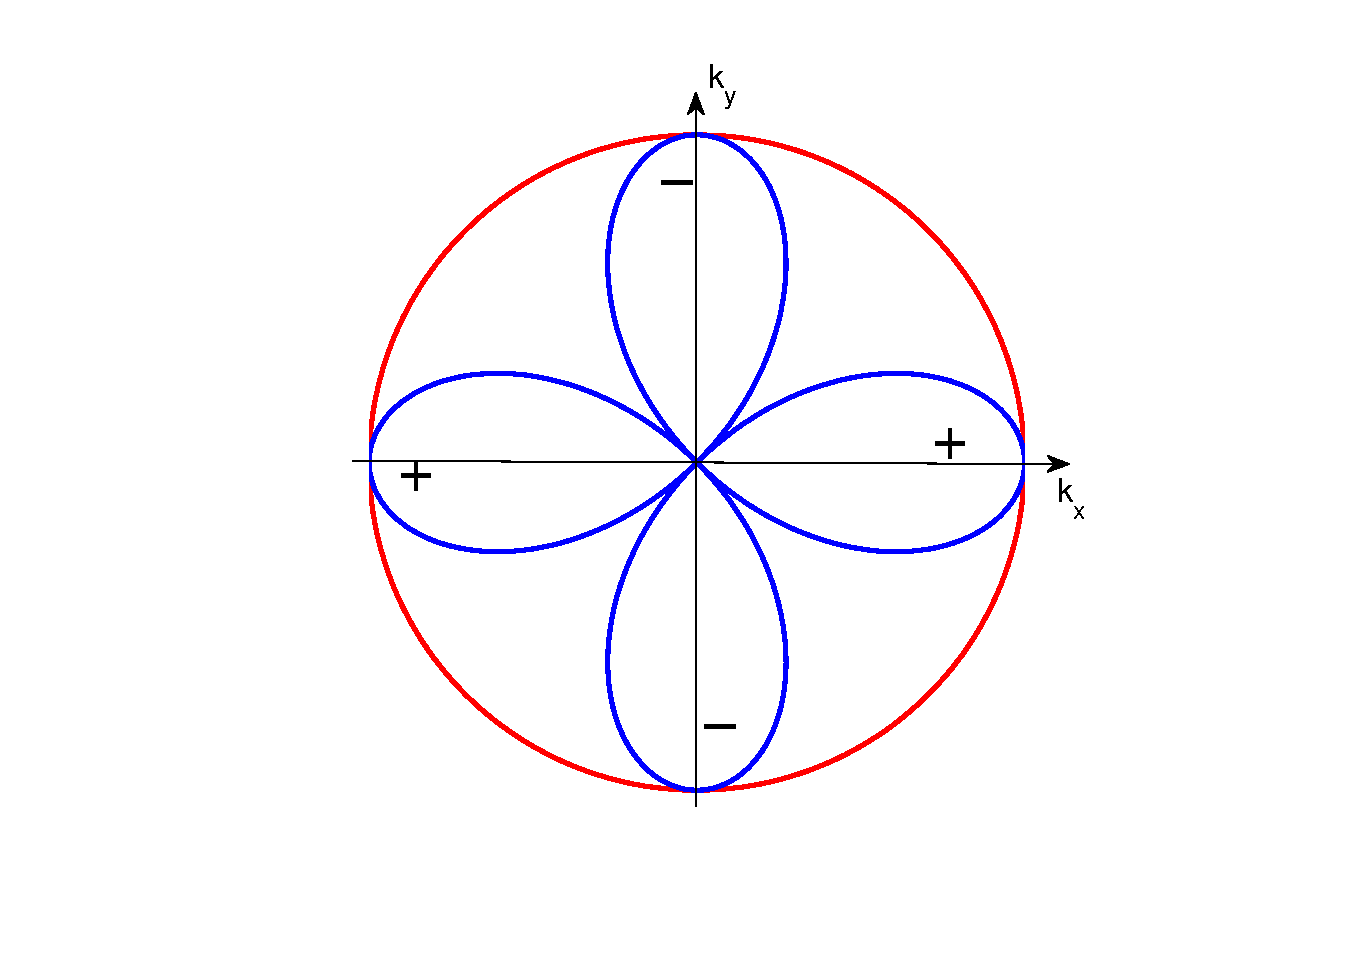
\includegraphics[width=10cm]{./Figures/2-1-1.eps}
\rule{35em}{0.5pt}
\caption[An Electron]{The shape of s-wave energy gap is a circle while that of d-wave energy gap is like a petal. Notice that the $d_{x^2-y^2}$ has two positive and negative leaves}
\label{Pair Potential Fig}
\end{figure}

\section{$D$-Wave Tunnelling Spectroscopy of Superconductors}
To approach the calculation of tunnelling spectroscopy of superconductors to fit the experimental results in our group, there are several steps to go in both theory and calculation. First of all, we need to establish the model for $s$-wave, the basis for the following calculations. Second, $s$-wave model serves the kernel so that it will guide us to the d-wave tunnelling spectroscopy results by conducting an integral over it. Finally, we obtain the conductances that can be compared to our BSCCO on BSC experiments. In addition, an algorithm for fitting the results is implemented.

We first introduce the formula for the conductance versus bias\citep{Reference6} before we discuss  the details of the d-wave tunnelling spectroscopy.  
\subsection{I-V Curve Function For N-S Boundary}
The reference\citep{Reference6} derives that the I-V curve for N-S Boundary could be written like
\begin{eqnarray}\label{BTK Conductance}
I_{NS}=2N(0)ev_F\mathcal{A}\int_{-\infty}^{\infty}[f_0(E-eV)-f_0(E)][1+A(E)-B(E)]dE
\end{eqnarray}
in which $f_0(E)$ is the fermi distribution and B(E) is the probability of normal reflection and A(E) is the probability of Andreev reflection, namely where the electron enters the superconductor as a cooper pair, while reflecting a hole.
\begin{eqnarray}
f_0(E) = \DF{1}{1+e^{(E-\mu)/kT}}
\end{eqnarray}
where $\mu$ is the chemical potential. 
By applying a differential operation on \eqref{BTK Conductance} we get that
\begin{eqnarray}\label{Conductance}
\sigma=\frac{\partial I}{\partial V}=\int_{-\infty}^{\infty}\sigma_T(E)\frac{\partial{f_0(E-eV)}}{\partial{V}}dE
\end{eqnarray}
Omitting the constant factor, the following term is what we are focusing on
\begin{eqnarray}\label{2D-Kernel}
&&\sigma_T(E) = \int d\Omega\sigma_S\cos\theta=\int d\Omega(1+A(E)-B(E))\cos\theta\nonumber\\
&&\sigma_S(E)=1+A(E)-B(E)
\end{eqnarray}
where $A(E)$ is the famous Andreev reflection and $B(E)$ is the ordinary reflection, and $\theta$ is the incident angle since we are only considering the current along the tunnelling axis\citep{Reference6}, the former of which reflects a hole and generate a Cooper pair in the superconductor side.

\subsection{Properties of Tunnelling Spectroscopy Kernel $\sigma_S$}
Let's first study the tunnelling spectroscopy kernel $\sigma_S$ shown in \eqref{2D-Kernel}.

The Bogoliubov equations can be analytically solved if we assume that the potential between the two materials is a $\delta$ function while energy gap is a step function \citep{Reference2}, demonstrated in Fig.\ref{fig:BTK Pair Potential}.
\begin{figure}[htbp]
\small
\centering
\includegraphics[width=10cm]{./Figures/2-2-1.eps}
\rule{35em}{0.5pt}
\caption[An Electron]{$\delta$ function of potential and step function of energy gap}
\label{fig:BTK Pair Potential}
\end{figure}
Also we define the effective pair potential $\Delta_+$ felt by the electron-like particles and effective pair potential $\Delta_-$ felt by the hole-like particles as following

\begin{eqnarray}\label{General Phase Pair}
\Delta_{\pm}=|\Delta_{\pm}|\exp(i\phi_{\pm})
\end{eqnarray}
From the analytical solutions of BdG equations, we obtain the kernel of \eqref{2D-Kernel}, which is written in \eqref{1DKernel}.
\begin{eqnarray}\label{1DKernel}
\sigma_R(E)=\frac{\sigma_S(E)}{\sigma_N}=\frac{1+\sigma_N\mid\Gamma_+\mid^2+(\sigma_N-1)\mid\Gamma_+\Gamma_-\mid^2}{\mid1+(\sigma_N-1)\Gamma_+\Gamma_-\exp(i\phi_--i\phi_+)\mid^2}
\end{eqnarray}
where the terms $\Gamma_{\pm}$,the normal conductance $\sigma_N$ and the effective barrier hight $Z$ are
\begin{eqnarray}
\Gamma_{\pm}=\frac{E-\sqrt{E^2-|\Delta_{\pm}|^2}}{|\Delta_{\pm}|},Z=\frac{Z_0}{\cos\theta},
\sigma_N=\frac{1}{1+Z^2}
\end{eqnarray} 
and we write the term $\sigma_S(E)$ for convenience.
\begin{eqnarray}\label{Tanaka Kernel}
\sigma_S(E)=\sigma_N\frac{1+\sigma_N\mid\Gamma_+\mid^2+(\sigma_N-1)\mid\Gamma_+\Gamma_-\mid^2}{\mid1+(\sigma_N-1)\Gamma_+\Gamma_-\exp(i\phi_--i\phi_+)\mid^2}
\end{eqnarray}
Fig.\ref{fig:Kernel Vary Z} indicates different shapes with different, $Z$, the barrier hight, where we assume that the phase difference $\phi_--\phi_+=0$.

\begin{figure}[htbp]
\small
\centering
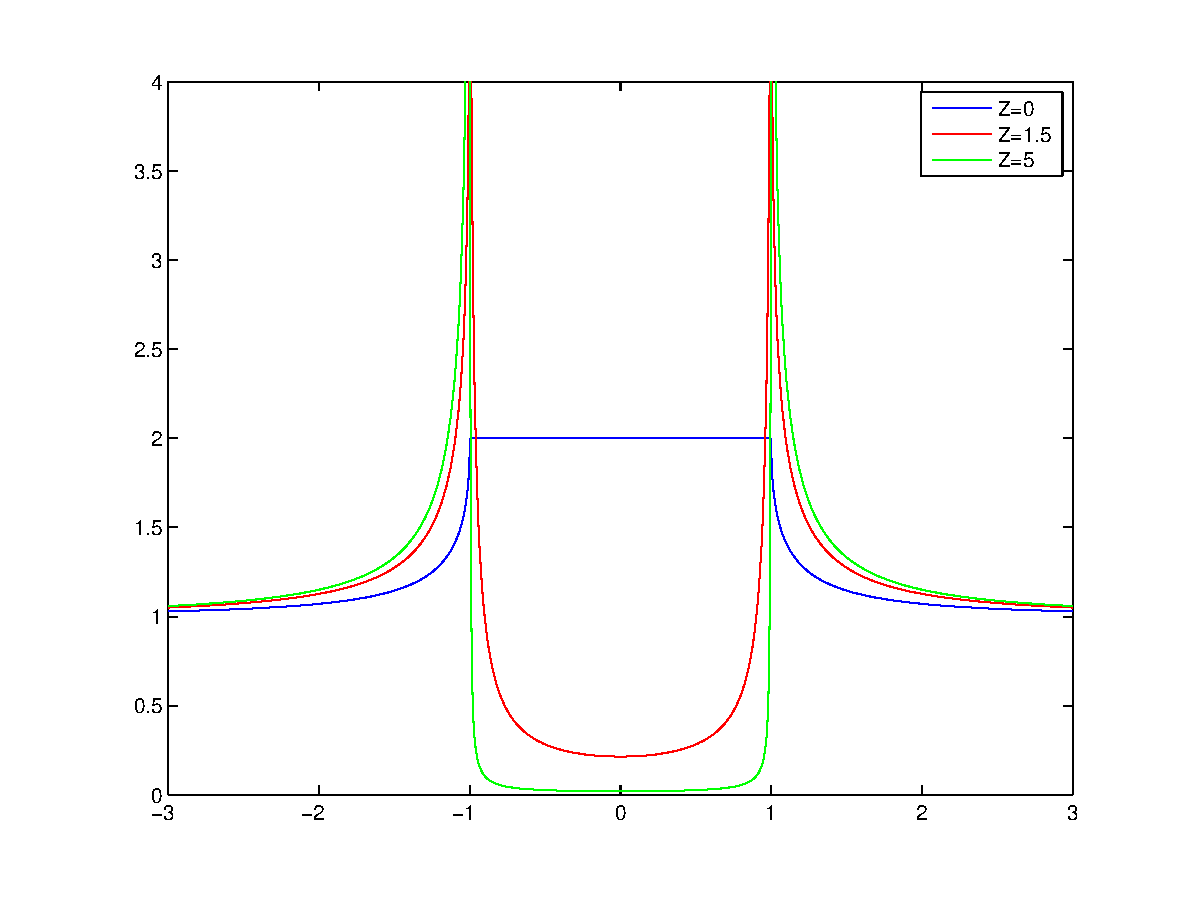
\includegraphics[width=10cm]{2-2-2.eps}
\caption{The picture indicates the different shapes of $\sigma_R(E)$ corresponding to the different barrier values. Here $\Delta_+=\Delta_-$}
\label{fig:Kernel Vary Z}
\end{figure}

The general function for the normalised tunnelling conductance $\sigma_T$ is 
\begin{eqnarray}\label{2D-Kernel-Integral}
\sigma_T(E)=\DF{\int d\Omega \sigma_S(E)\cos\theta}{\int d\Omega\sigma_N\cos\theta}
\end{eqnarray}
where we can see that the kernel $\sigma_S$ is implemented.
The integral operators in $d$-wave $ab$ tunnelling and in $c$-tunnelling is written as
\begin{eqnarray}\label{abc}
&&\int d\Omega^{(ab)}=\int_{-\pi/2}^{\pi/2} d\theta\nonumber\\
&&\int d\Omega^{(c)}=\int_{0}^{2\pi}d\varphi\int_{0}^{\pi/2} d\theta \sin\theta
\end{eqnarray}
$\varphi$ is the interface angle.

\subsection{$ab$-Tunnelling Spectroscopy}
The $d$-wave tunnelling spectroscopy has are two cases: $ab$ tunnelling whose tunnelling axis is normal to the $c$-axis of the crystal, and $c$ tunnelling whose tunnelling axis is parallel to the $c$-axis of the crystal, Fig.\ref{Pair Potential Fig}. We first of all discuss $ab$-tunnelling spectroscopy.

In fact, the averaged normal conductance in \eqref{2D-Kernel-Integral} can be derived directly.
\begin{eqnarray}
\overline{\sigma_N}=\int d\Omega^{(ab)} \sigma_N\cos\theta
\end{eqnarray}
so that
the averaged normal conductance is
\begin{eqnarray}
\overline{\sigma_N}=2-\frac{Z_0}{\sqrt{1+Z_0^2}}\ln\Big(\frac{\sqrt{1+Z_0^2}+1}{\sqrt{1+Z_0^2}-1}\Big)
\end{eqnarray}

Now we focus our discussion on the specific case of $d_{x^2+y^2}$, where in $ab$-tunnelling $\Delta_-,\Delta_+$ are written as
\begin{eqnarray}\label{ab pair potential}
\Delta_+=\Delta_0\cos2(\theta-\alpha)\nonumber\\
\\
\Delta_-=\Delta_0\cos2(\theta+\alpha)\nonumber
\end{eqnarray}
where $\theta$ represents incident angle, $\alpha$ the angle between the tunnelling axis and main axis of the pair potential, shown in Fig.\ref{fig:ab-tunnelling schematic}.
\begin{figure}[htbp]
\small
\centering
\includegraphics[width=10cm]{ab-tunnelling.eps}
\caption{Schematic illustration of the incident angle $\theta$ and the angle $\alpha$.}
\label{fig:ab-tunnelling schematic}
\end{figure}


Turning to Fig.\ref{fig:dc-alpha}, we see the shape of the conductance is sensitive to the incident angle and thus the phase difference 
\begin{eqnarray}\label{d wave phase difference}
e^{i\phi_--i\phi_+}=\frac{|\Delta_+|}{\Delta_+}\frac{\Delta_-}{|\Delta_-|}=\frac{|\cos2(\theta-\alpha)|}{\cos2(\theta-\alpha)}\frac{\cos2(\theta+\alpha)}{|\cos2(\theta+\alpha)|}\in\{-1,1\}
\end{eqnarray}

\begin{figure}[htbp]
\small
\centering
\includegraphics[width=10cm]{2-2-5.eps}
\caption{The figure indicates the correspondence of conductance and angle between incident normal and the petal axis.}
\label{fig:dc-alpha}
\end{figure}

Furthermore we limit the phase difference to zero. 

Fig.\ref{fig:dc-gap} shows the property of the $ab$ tunnelling spectroscopy respect to different pair potentials, which indicates that one pair potential corresponds to one peak in the figure, while if pair potential is zero, the tunnelling conductance is a constant, $1$.
\begin{figure}[htbp]
\small
\centering
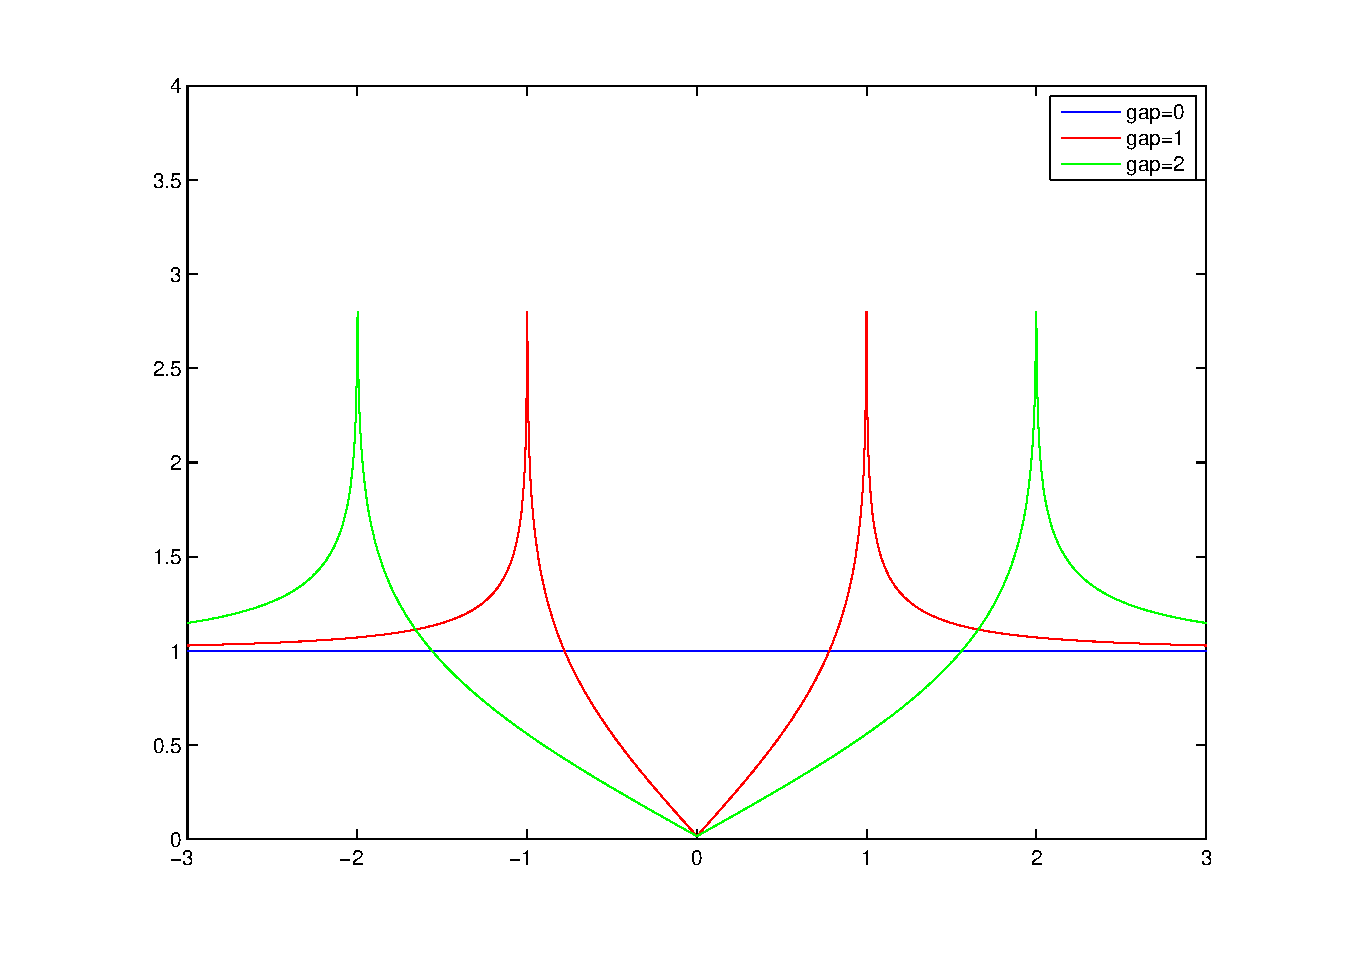
\includegraphics[width=10cm]{2-2-4.eps}
\caption{The figure demonstrates the total tunnelling conductance with different
energy gaps. When energy gap amplitude is zero, the peaks vanish, meaning
that the material turns into normal metal. Here we choose $Z=5$}
\label{fig:dc-gap}
\end{figure}

\subsection{Differential Conductance with Different Temperatures and Fixed Energy Gap Amplitude}
In general, the properties of differential conductance is determined by the derivative of the fermi function and tunnelling conductance kernel, according to \eqref{Conductance} and \eqref{1DKernel}.
As an illustration,Fig.\ref{fig:fermi-dc} shows differential conductance at Temperature 1K, where the top figure is the differential conductance, the bottom figure is the tunnelling conductance, and the others are the derivatives of fermi function at different biases. We see that the peak of the derivatives are close to $\delta$ functions, which makes the differential conductance look similar to the tunnelling conductance after the integration.
\begin{figure}[htbp]
\small
\centering
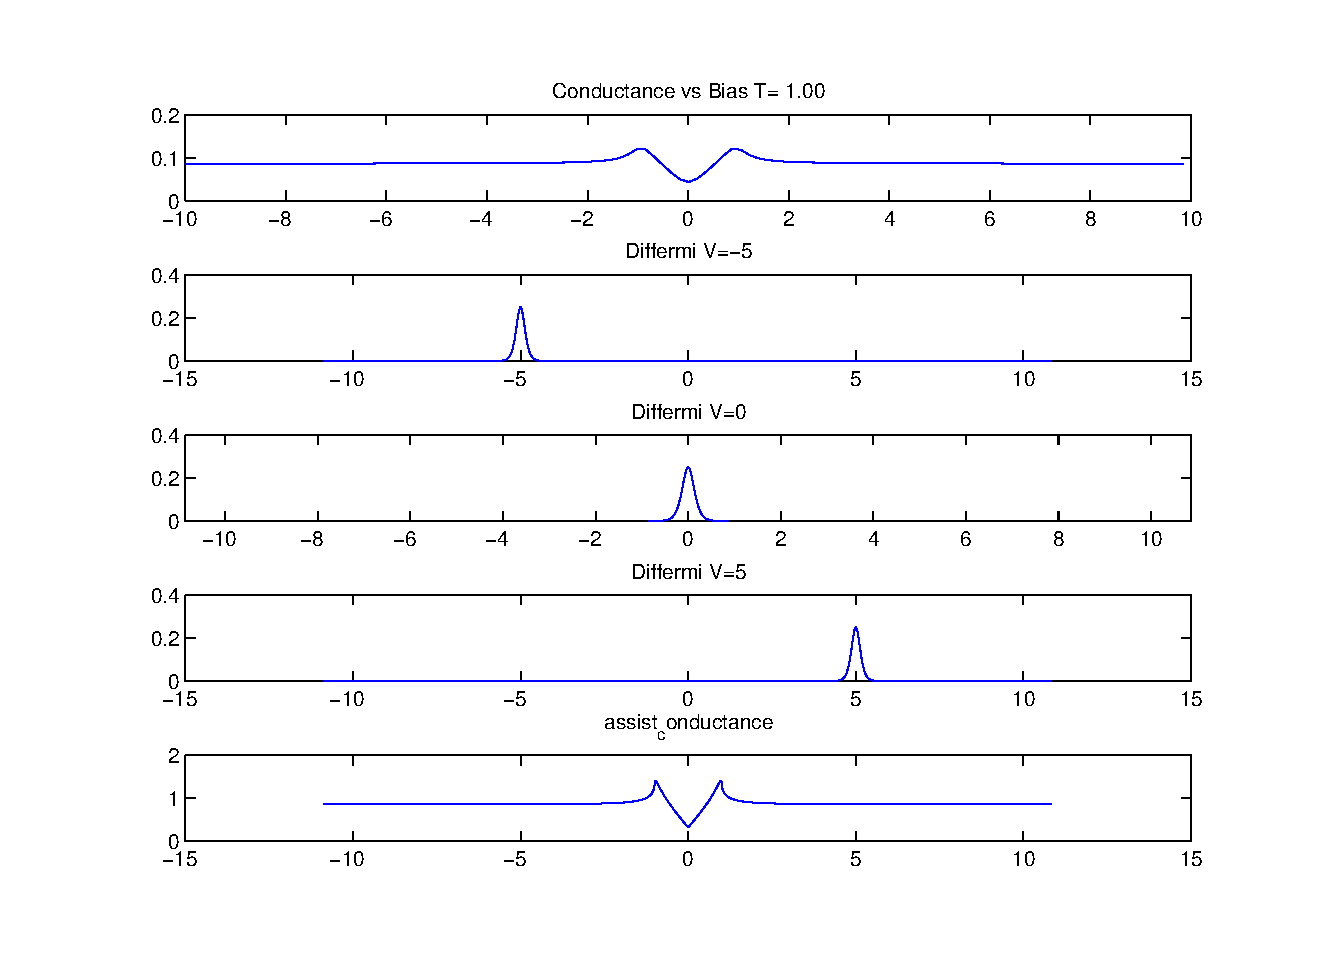
\includegraphics[width=12cm]{2-2-6.eps}
\caption{Differential conductance with T=1K, accompanied by plots of three derivatives of the fermi distributions at varied biases and  a tunnelling conductance graph in the bottom.}
\label{fig:fermi-dc}
\end{figure}

Let's discuss a way to make the picture more clear in Fig.\ref{fig:3D-dc}, demonstrating the relation between the tunnelling conductance with temperature with a FIXED pair potential. We could observe that the dip in middle generally vanish as the temperature increases.
\begin{figure}[htbp]
\small
\centering
\includegraphics[width=12cm]{2-2-8.pdf}
\caption{This figure indicates the relation between temperature, bias and the conductance.The different colours indicate the temperature.}
\label{fig:3D-dc}
\end{figure}

\subsection{Differential Conductance with Different Pair Potential Amplitudes with Fixed Temperature}
Though we should be clearly warned that the energy gap is dependent on the temperature, we still do a study for the relation between differential conductance with energy gap amplitudes.

Generally, the shapes of tunnelling conductance are similar except when the energy gap amplitude is zero, which will make the tunnelling conductance constant, already indicated in Fig.\ref{fig:dc-gap}.

Therefore, we simply provide an illustration figure. We could notice that with the increase energy gap amplitude, the centre dip becomes deeper, Fig.\ref{fig:3D-dc-gap}.
\begin{figure}[htbp]
\small
\centering
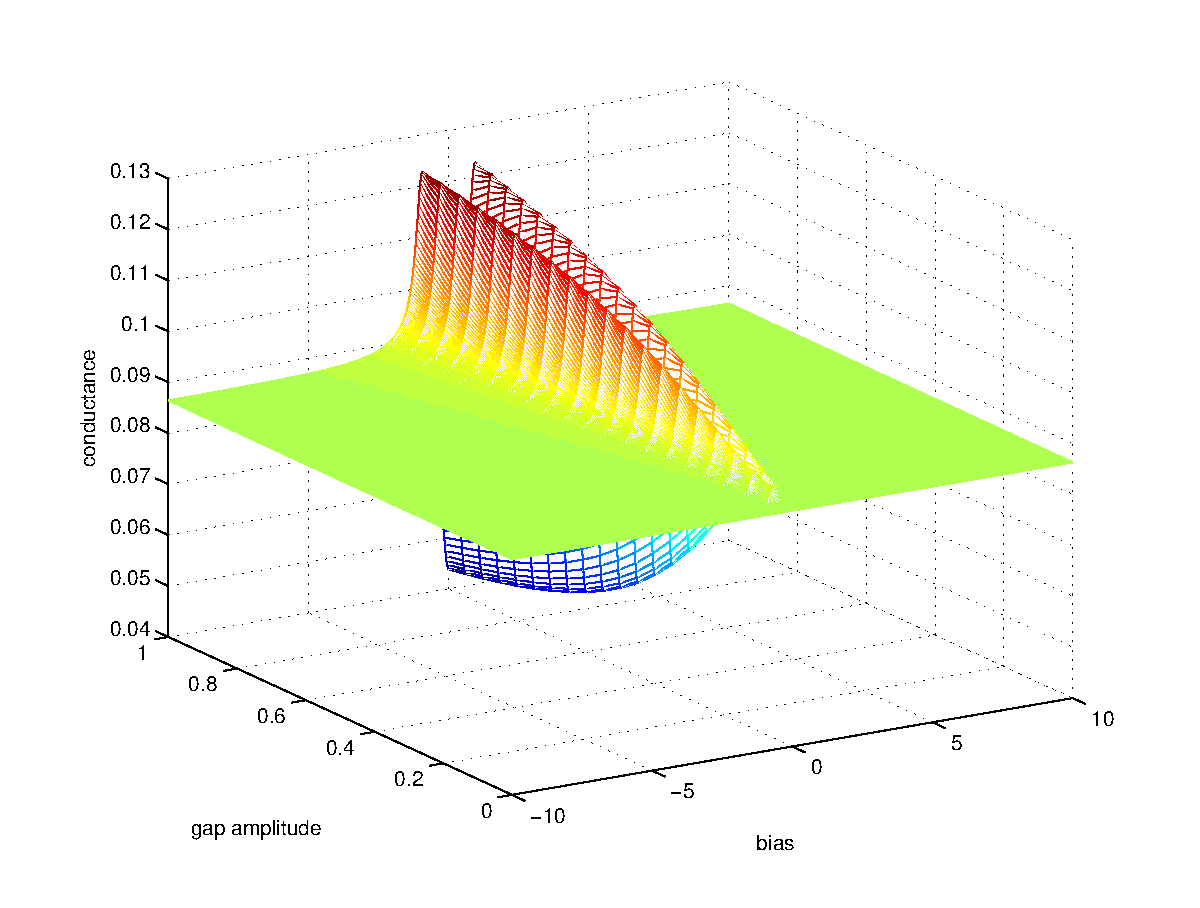
\includegraphics[width=12cm]{2-2-9.eps}
\caption{This figure indicates the relation between energy gap amplitude, bias and the conductance.}
\label{fig:3D-dc-gap}
\end{figure}


Now we briefly introduce the calculation methods. It should be noted that we are trying to calculate a second order integral, which may lead to a large calculation time, as that we might have to calculate $1000\times1000$ volume. I developed a simple method based on the essential features of function $\sigma_S$ and differential fermi distribution function $\frac{\partial{f_0(E-eV)}}{\partial{V}}$ in the integrations\eqref{Conductance} and \eqref{2D-Kernel-Integral}.

First of all, the function $\sigma_T(E)$ is assumed to be  CONSTANT when parameter E's absolute value is to some extent larger than amplitude of the energy gap, Fig.\ref{fig:dc-gap}.

Second, we note that differential fermi distribution function is actually of Delta function type, which means the value could be assumed zero when its parameter $E-\mu-eV$ is "much" larger than $kT$. Also, all the derivatives of the fermi distribution function shares the exact shape, shown in Fig.\ref{fig:fermi-dc}; their only difference is that the peaks are in different positions corresponding to the value of bias.

With the above knowledge, we calculate the the tunnelling spectroscopy point values according to a chosen step length ONLY ONCE and store the data. When parameter $E$ is "large", we use constant for the point. We define this as calculation (1).
Also, we calculate the point values of the derivative of the fermi distribution function at bias zero according to the step length used in the calculation (1). When parameter $E-\mu-eV$ is "large", we make the point value as zero. When We define this as calculation (2).
Since calculation (1) and calculation (2) share the same step length, if we need to calculate the differential conductance at a certain bias, we translate the point values of the derivative to that bias and do the integration limited to the non-zero points of the derivative.
To avoid losing information, the choice of the step length is significant. We choose step length according to the smaller value of peak width between the differential fermi distribution function and tunnelling conductance.
The method remarkably improves the performance of the calculation yet loses very little accuracy. The weakness of this method is that the computation is slow when energy gap amplitude is small while the temperature is high, which, however, is easily to be removed by adding some plotting and integrating step boundaries.

\subsection{$c$-Tunnelling Spectroscopy and Fitting the Experimental Data}
As our experiments are conducted with the materials along $c$-axis of d-wave pair potential, we now focus on this case. The schematic illustration is shown in Fig.\ref{fig:c-tunnelling schematic}.
\begin{figure}[htbp]
\small
\centering
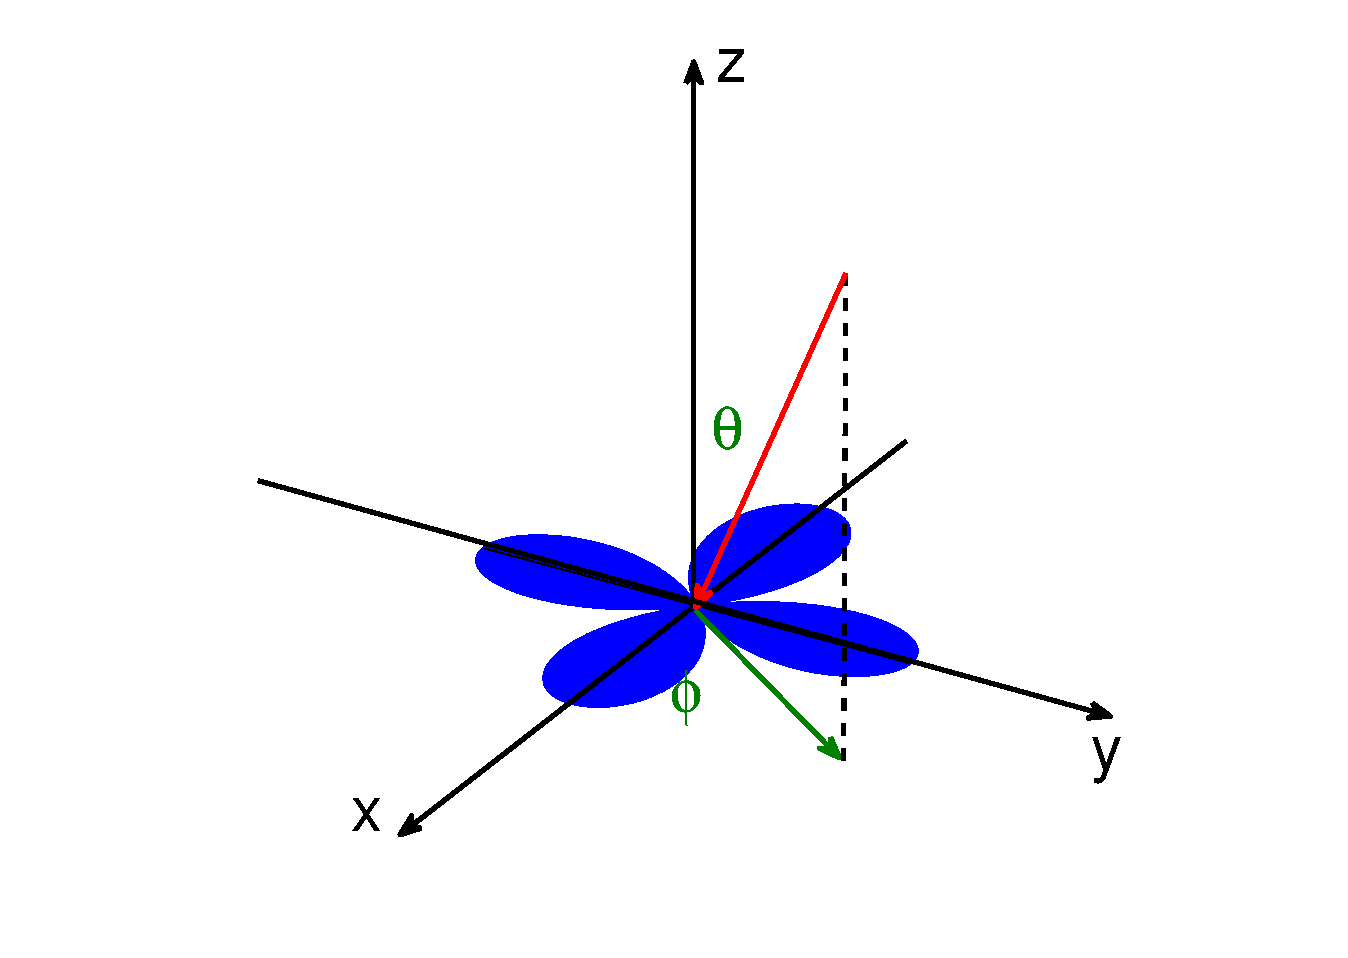
\includegraphics[width=12cm]{./Figures/c-tunnelling.eps}
\caption{The schematic illustration of $c$-tunnelling, where the incident angle $\theta$ and the interface angle $\varphi$ are indicated. In the figure, $x-y$ plane is the tunnelling interface.}
\label{fig:c-tunnelling schematic}
\end{figure}
The pair potential in $c$-tunnelling is written as
\begin{eqnarray}
\Delta(\varphi)=\Delta_0\cos2\varphi
\end{eqnarray}
The averaged N-I-N junction conductance over the half-sphere of $k$ space could be calculated directly.
According to the formula in the following, that calculates the averaged normal conductance,
\begin{eqnarray}
\overline{\sigma_N}=\int_0^{2\pi}d\phi \int_{0}^{\frac{\pi}{2}} d\theta \cos\theta\sin\theta \sigma_N
\end{eqnarray}
where we assume that 
\begin{eqnarray}
\sigma_N=\DF{1}{1+(\DF{Z_0}{\cos\theta})^2}
\end{eqnarray}
We could simply calculate the integral for averaged normal conductance,
\begin{eqnarray}\label{average-normal}
\overline{\sigma_N}=\pi \Big[1-Z_0^2\ln\Big(1+\DF{1}{Z_0^2}\Big)\Big]
\end{eqnarray}
Knowing the formula \eqref{average-normal}, we could step over the numerical integral of normal conductance. Ideally, it also can be used to calculate the barrier hight.
 
Typically the $c$-tunnelling spectroscopy is similar to that of $ab$-tunneling, when alpha = 0, since the incident angle averages over the d-wave gap in a similar manner. 

We conducted an experiment about the tunnelling spectroscopy with the layers of the material Bismuth strontium calcium copper oxide having the generalised chemical formula $Bi_2Sr_2Ca_{n-1}Cu_nO_{2n+4+x}$ (BSCCO) and Calcium doped $Bi_2Se_3$(BSC), the former of which serves as a cuprate superconductor \citep{BSCCO} and the latter of which serves as a topological insulator\citep{Semiconductor}. We use $d$-wave $c$-tunnelling model to fit the experimental data.
Fig.\ref{fig:fitting} shows the fitting results for our BSCCO on BSC experimental results by manually inputting the parameters.
 \begin{figure}[htbp]
\small
\centering
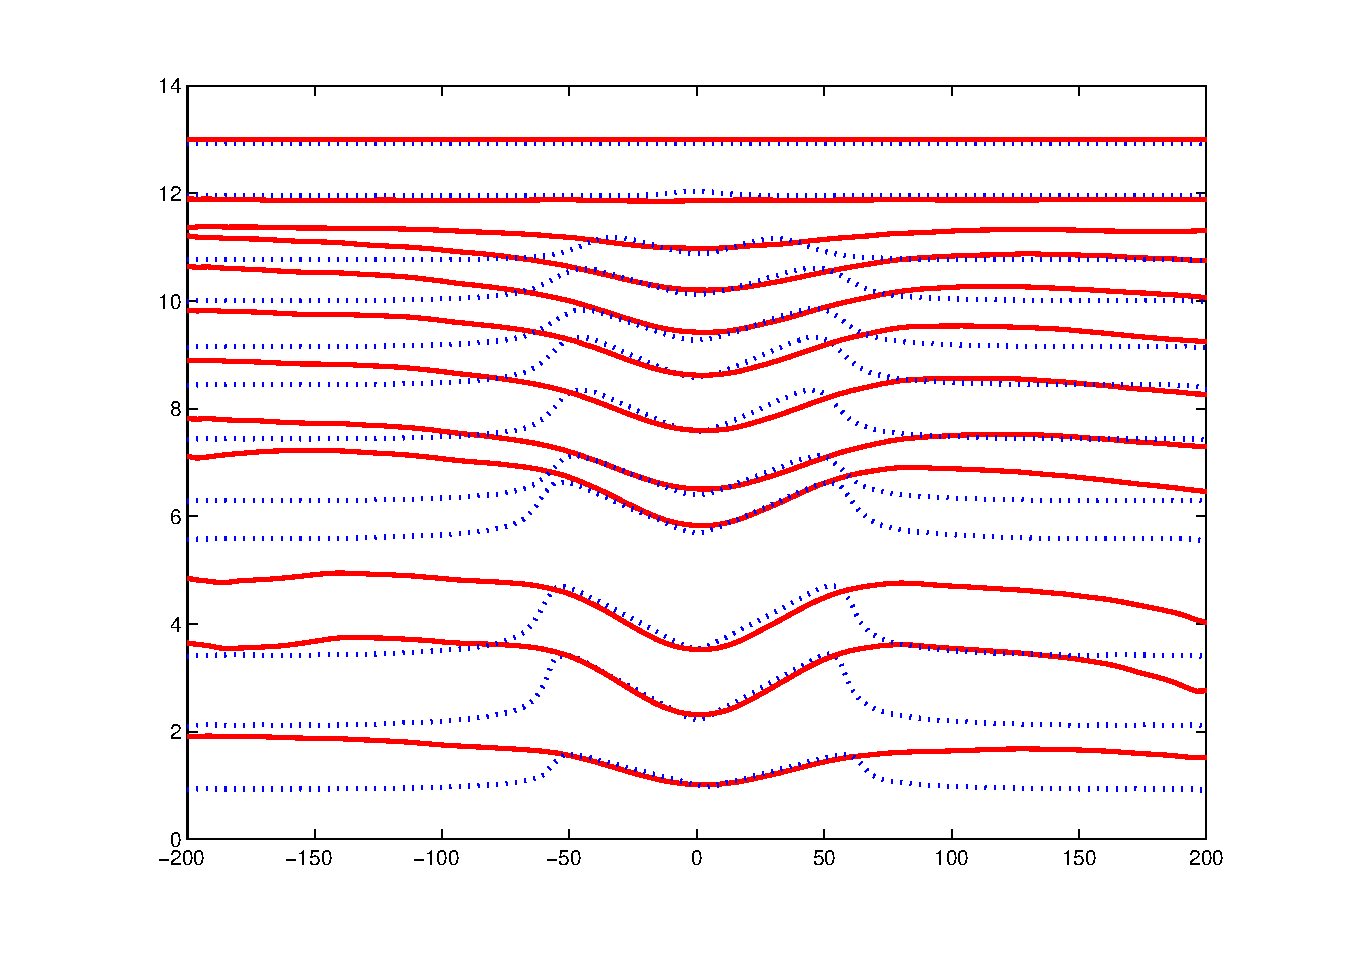
\includegraphics[width=12cm]{./Figures/Fitting.eps}
\caption{Conductances normalised by 70K with Temperature, where the deep colour represents calculation. Each bundle represents, from bottom to top, sequentially,  $10K$,$13K$,$15K$,$30K$,$35K$,$40K$,$45K$,$50K$,$55K$,$65K$,$70K$.}
\label{fig:fitting}
\end{figure}

And chosen energy gaps versus temperature for fitting the experimental data are shown below, Fig.\ref{fig:fit pair potential}.
 \begin{figure}[htbp]
\small
\centering
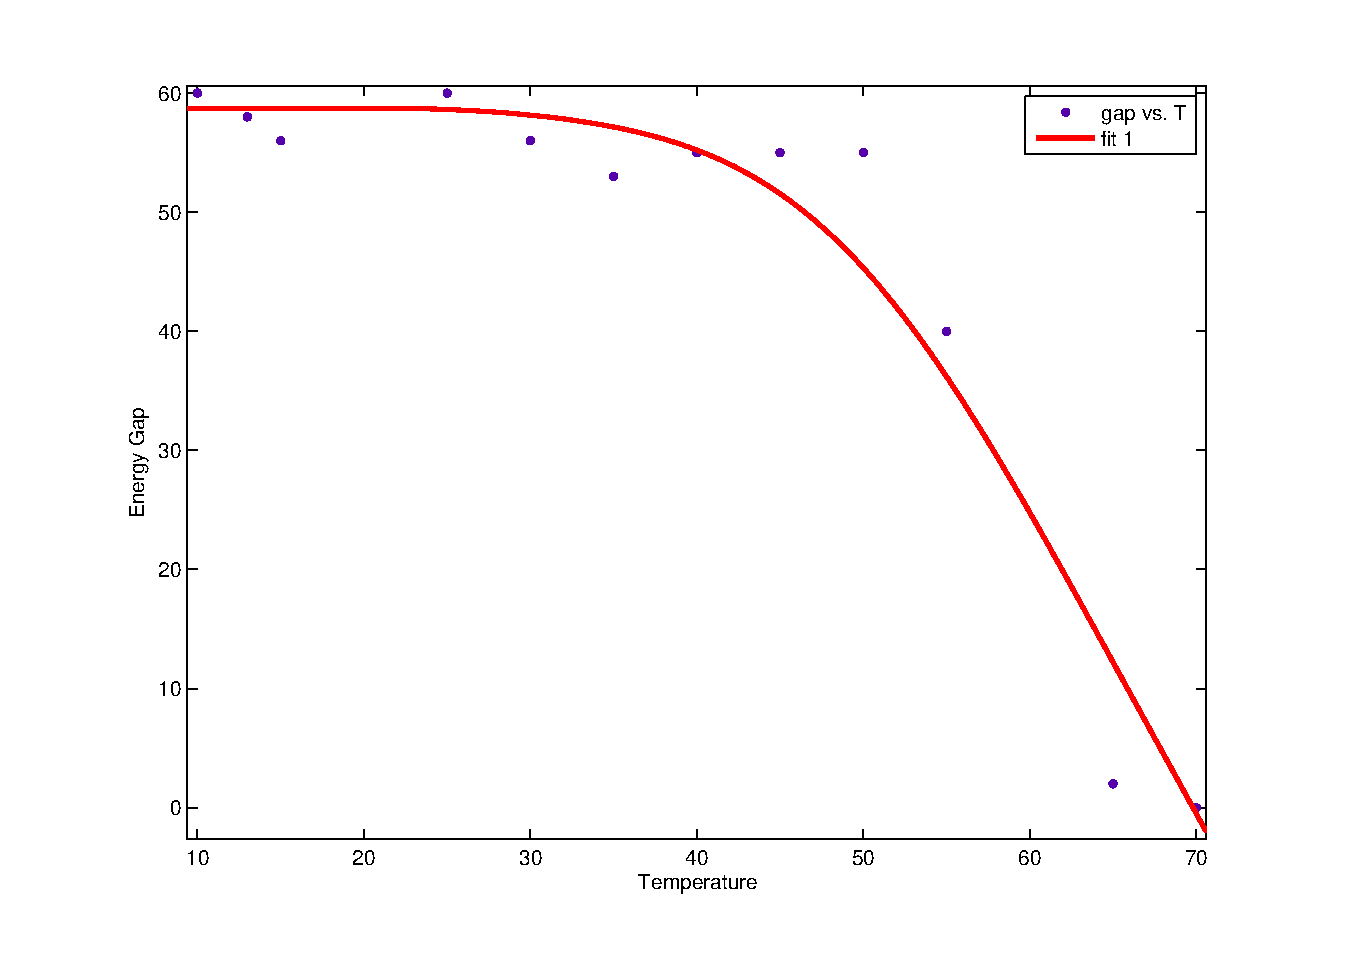
\includegraphics[width=8cm]{gap.eps}
\caption{Energy Gaps with Temperature}
\label{fig:fit pair potential}
\end{figure}


The fitting results are not satisfactory. Only in the dip part the fitting results agree to some extent with the experimental results. But at the both sides they are quite far away. The reason for this disagreement is that the model we use is for low temperature case and is based on the assumption that the density of states is a constant at (2.12) and the properties of our model is determined by the integration kernel of (2.19), which also has peaks at the point $E=\Delta_0$. The experiment results, however, do not have the corresponding peaks, leading to the fact that the fitting results only match a small part of the experimental results in the centre.

To try to eliminate of the disagreement from the computational part, we implemented the genetic algorithm for fitting the data\citep{GA}.

Genetic algorithm(GA) is an optimisation heuristic inspired by the natural selection process in biological systems. Very similar to the selection process, GA maintains a population of candidates and process mechanisms of encoding, selection, crossover, mutation and culling in the population\citep{GA}. 

In the calculation, we select a population of 50 for the desired parameters randomly generated within the set range and calculate the fitness value, such as standard error and then sort the population according to the fitness value increasingly. Second, we choose the first 25 of the population according to the sorted list as parents while we select another 25 samples of the population as mutants randomly multiplied by some restricted random numbers. 25 selected parents will generate 25 offsprings by crossover. Then we mix the original population, the generated offspring as well as the 25 mutants together to compose a country of 100 samples. Third, we do sorting again with the population the eliminate the last 50 samples of the population. We will repeat the above three steps until the termination requirement is satisfied. 

The above statement is the ideal approach to fit the experimental data, while unfortunately the results come out not satisfactory.










































